\documentclass[14pt]{extarticle}
\usepackage[utf8]{inputenc}
\usepackage[T1]{fontenc}
\usepackage[ngerman]{babel}
\usepackage{array}
\usepackage{amsmath}
\usepackage{graphicx}
\title{Bericht Todesstern U4}
\author{Charline Waldrich, Robert Ullmann, Julian Dobrot}
\date{12. Dezember 2015}

\begin{document}

\maketitle
\pagebreak
\tableofcontents


\section{Aufgabenstellung}
Implementierung von Schatten und Reflexion in der Beleuchtung des Todesstern Raytracers.
\subsection{Änderungen an bestehenden Klassen}
Die abstrakte Oberklasse Light wurde um das boolean Attribut castsShadows erweitert. Außerdem wurde die Illuminates Methode um den Parameter World erweitert, da es so möglich ist zu ermitteln ob ein Objekt zwischen den der Lichtquelle und dem anderen Objekt steht. \\
Außerdem erhaelt die Methode colorFor als zusaetzlichen Parametern einen Tracer. 
\subsubsection{Neue Klassen}
Ein Tracer ist ein Objekt, welches eine Funktion zum Raytracen zur Verfuegung stellt (die Funktion fr(r)). \\
Des weiteren kommt ein neues Material namens ReflectiveMaterial hinzu.

Die Klasse Geometry bekommt nun das Material übergeben, welches in der Materialklasse die Methode colorFor aufruft. 

\section{Implementierungen}
Die Tracer Klasse bleibt vorerst leer. 
Die ReflectiveMaterial Klasse basiert auf der mathematischen Formel fuer einen perfekt diffus reflektierenden Koerper mit einem Glanzpunkt und Reflektion.
$
c = c_d c_a + \sum_{i=1}^i_max [ c_d * c_l * max(0, \vec e . \vec r_l )^P ] + c_r f_r [ ( \vec p_r , \vec r_d ) ] 
$
Diese wurde in der colorFor Methode der Klasse in einen Code umgewandelt welcher stets die Farbe diffus reflektierenden Objektes direkt zurueck gibt und gleichzeitig die Funktion des Tracers mit den Koordinaten dessen Reflexion aufruft damit der Schatten erzeugt werden kann.

\section{Testszenen}

Drei Kugeln mit reflexivem Material in unterschiedlichen Farben auf Schwarzem Hintergrund. 
\begin{figure}[ht]
\begin{center}
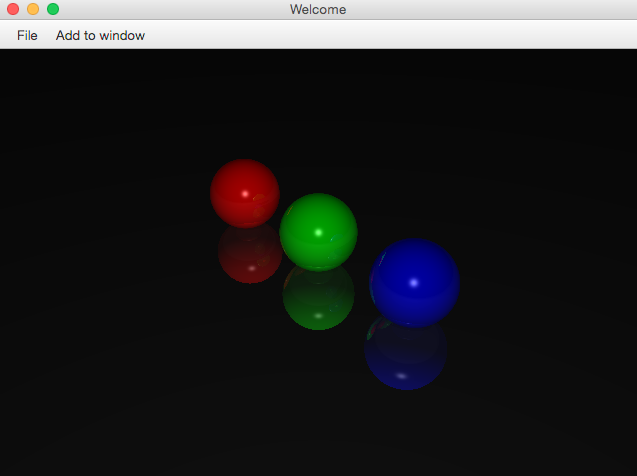
\includegraphics[scale=10]{images/Szene1.png}
\caption{Szene 1}
\label{Szene 1}
\end{center}
\end{figure}

Eine rote Box auf einer Ebene mit grau reflektierendem Material.
\begin{figure}[ht]
\begin{center}
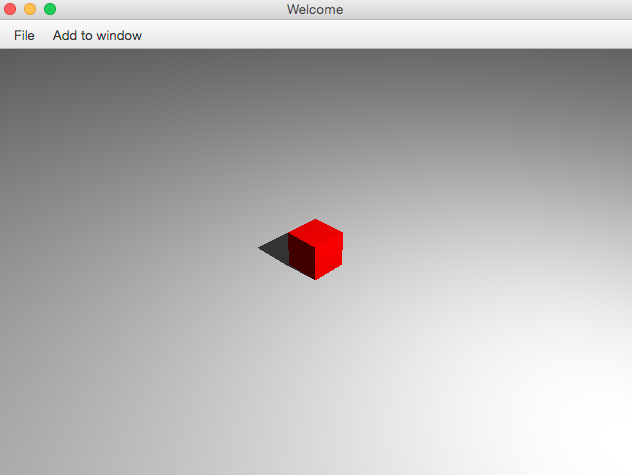
\includegraphics[scale=10]{images/Szene2.png}
\caption{Szene 2}
\label{Szene 2}
\end{center}
\end{figure}


\section{Zeitbedarf}
\begin{center}
\begin{tabular}{cr}
Änderungen an bestehenden Klassen \	&60 min	\\
Licht	  \	&240 min	\\
Material 	\	&180 min	\\
Welt \	&60 min	\\
Demo \	&240 min	\\
Bericht  \		&180 min	 \\
	\hline
	&960 min
\end{tabular}
\end{center}

\section{Quellen}

\end{document}
